\title{Metamorph User Guide}
\author{Markus Michael Geipel}
\date{\today}

\documentclass[12pt,a4paper]{article}

\usepackage{a4wide}
\usepackage{cite,graphicx}
\usepackage{amssymb}
\usepackage{listings}
\usepackage{caption}
\usepackage{draftwatermark}
\usepackage{relsize}
\usepackage{hyperref} 

\SetWatermarkScale{5}

%\usepackage{color}
%\definecolor{gray}{rgb}{0.4,0.4,0.4}
%\definecolor{darkblue}{rgb}{0.0,0.0,0.6}
%\definecolor{cyan}{rgb}{0.0,0.6,0.6}


\lstloadlanguages{XML}
\lstset{
language=XML,
basicstyle=\small\sffamily\smaller,
frame=tb,
%framexleftmargin=6px,
%framexrightmargin=6px,
columns=fullflexible,
captionpos=b,
}


\begin{document}
\maketitle

\begin{abstract}
Metamorph is a Java library including an XML based data transformation language, designed to ease dealing with metadata. In this document the design rationale behind Metamorph is discussed, followed by a user guide including many hands-on code examples. As a conclusion several real-world application scenarios are presented.
\end{abstract}

\setcounter{tocdepth}{2}
\tableofcontents

\section{Introduction}
Metadata is a central ingredient of any information storage and retrieval system. Being defined as ``data on data'', metadata provides descriptive information on the items stocked in the system; be it a library, an archive, a museum or a web search engine.

The variety of possibly stored items is reflected in the plethora of existing metadata formats. Obviously, a museum needs to describe its exposition items differently than a library its available books. And even the same book may be described differently depending on the institution holding it: A library has different description needs than a book seller. The first might use a standard such as Marc 21, the latter might use ONIX. Furthermore, standards also differ depending on the country or the language. Finally new technologies bring up new information needs not reflected in existing standards. 
%New standards addressing the needs of the electronic age include for instance Dublin Core, METS and MODS.

In the face of a babylonic confusion of tongues, interoperability is an important issue, and metadata is transformed from one format to another on a regular basis. Transformations are not only performed to exchange data between institutions or to enable cross-collection searches. Metadata also needs to be transformed for indexing or for presentation in user-interfaces (on a webpage as HTML, for example). Despite being such an ubiquitous task, metadata transformation is still a tedious, mostly manual task, with scarce tool support. Software written to perform transformations is often coded from scratch for each and every individual case; despite great potential for component reuse. 

The purpose of this document is to explain how the metadata challenge is addressed by Metamorph, a Java library including a domain specific metadata transformation language expressed in XML. In the next section the classical metadata transformation process will be sketched to elucidate the inherent challenges and to motivate the requirements and design goals of Metamorph. Next, the general architecture will be presented, followed by a description of the language features. Metamorph was applied in various projects at the German National Library. In section \ref{apps} these application scenarios will be discussed.
A final section on the future prospects and limitations of Metamorph rounds up this document.


\section{Metadata Transformation in Practice}

Metadata transformation is a complex and sometimes tedious process as its correctness depends on an overlap of domain knowledge and programming skills. First the typical procedure will be skeched followed by a discussion of the resulting challenges.


\subsection{Workflow}

The first step is to create a Crosswalk or Conceptual Mapping between the two formats. Such a Conceptual Mapping normally consists of a table in human readable form and it is created and maintained by domain experts. Figure \ref{fig:mapping_simple} shows two simple mapping rules from Pica to RDF, taken from the DNB Linked Data Service. 

\begin{figure}[htp]
\centering
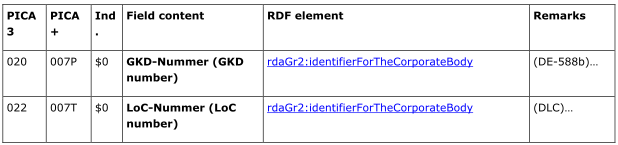
\includegraphics[width=.8\textwidth]{figures/mapping_simple}
\caption{Conceptual mapping for the DNB Linked Data Service}\label{fig:mapping_simple}
\end{figure}

On the left we see the respective fields in Pica, followed by an explanation of the content. Next, the target in RDF is defined, followed by remarks, indicating transformations applied to the data. The first line thus reads: Given a Pica+ recode, take the value of field {\tt 007P} subfield {\tt 0}, prepend {\tt (DE-588b)} and write it to the RDF element {\tt rdaGr2:identifierForTheCorporateBody}.  Figure \ref{fig:mapping_complex} shows a slightly more complex example. In this case values of different subfields need to be combined to fill the RDF element {\tt gnd:preferredNameForTheCorporateBody}. The last column defines this combination by reference to the subfield names.

\begin{figure}[htp]
\centering
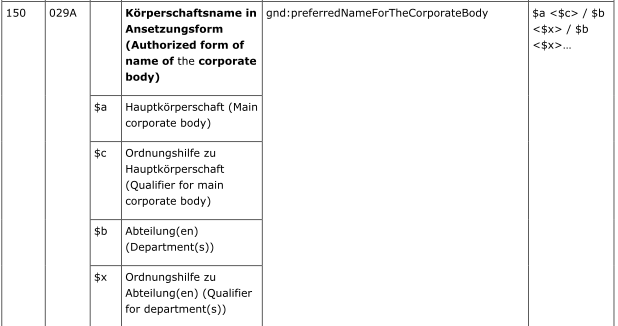
\includegraphics[width=.8\textwidth]{figures/mapping_complex}
\caption{A more complex mapping for the DNB Linked Data Service}\label{fig:mapping_complex}
\end{figure}



Based on the conceptual mapping, a piece of software is developed which implements the mapping. This is done by a programmer based the conceptual mapping document.



\subsection{Challenges}

The just described workflow poses several challenges which shall now be briefly discussed. In section \ref{arch} I will refer to them while introducing the architecture of Metamorph.

\subsubsection{From Concept to Code}

The transition forms the conceptual mapping to the actual code implementing it is a critical one. A conceptual mapping leaves space for interpretation. The programmer is the one to fill this gap, although he or she lacks the knowledge of the domain specialist.
Information flows one-way from domain specialist to programmer. What the programmer really implements cannot be double-checked by the domain specialist as he or she in turn lacks the fluency in the respective computer language the transformation is realized in.


\subsubsection{Format Independence}\label{format_ind}

Conceptual mapping between metadata schemata bear a lot of resemblance. The table structure in which the mapping is described is almost always the same. The software side implementing the mappings differs significantly, though. This is due to encoding details of the metadata formats. For instance the code and data structures or classes used load and represent Marc 21 records and pica records in a Java program differ, even though conceptually they are very similar. Both are composed of fields containing subfields. Slight differences in the implementations renders reuse of the code infeasible.


\subsubsection{Performance}

The input to a transformation from one format to another may well comprise millions of records. Performance is thus an issue. It is also important to note that transformations have to be performed repeatedly as the metadata keeps changing or errors in the mapping are discovered.

\section{Architecture}\label{arch}

This section introduces the general architecture of Metamorph, pointing out how it addresses the requirements of reusability, transparency and performance.

\subsection{Generic Data Structure}

At least in the library domain, the organization of the data within a record is fairly similar across formats (Marc, Pica and Mab2, for instance): A record consists of named fields, which in turn contain named subfields. The actual data is stored in these subfields. Many formats also store meta-information such as modification date in the record\footnote{Which would actually be meta-meta-data, to be precise.}. Metadata formats in the archive domain in turn tend to exhibit more hierarchical structures. As pointed out in section \ref{format_ind}, a common denominator is needed to enable code reuse. Metamorph thus makes the assumption that the structure depicted in figure \ref{fig:record2_class} may serve as such a common denominator. 
The structure is fairly general and allows also for hierarchical structures. It turns out that most data structures found in common metadata formats can be mapped to it easily.

In general {\tt Record} forms a self contained and independent unit. It may contain Literals or Entities which themselves may contain further Entities or Literals. A Field in library metadata (e.g. Pica) would map to an Entity, Subfields to Literals. The recursive organization of Entities whould not be called on in this case.
\begin{figure}[htp]
\centering
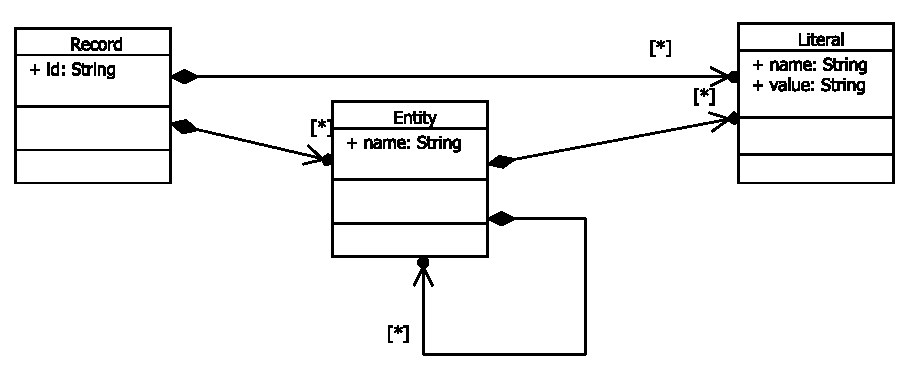
\includegraphics[width=.90\textwidth]{figures/record2_class}
\caption{The abstract data model underlying Metamorph}\label{fig:record2_class}
\end{figure}

The universality of data structure described in the previous section comes at a cost. To generate it explicitly is costly as it comprises many Java object such as literals, lists or maps, depending on the specific implementation. Handling such generic data structures normally results in convoluted if-infested code.
The solution to this dilemma is twofold: Firstly, as described in the next subsection we avoid ever explicitly instantiating the data structure in figure \ref{fig:record2_class}. Secondly, we use a domain specific language to handle transformation on the data stream, as sketched in subsection \ref{trans}.

\subsection{Data as a Stream of Events}

 Do we really need to explicitly construct the data structure for each record? No, it turns out that it can be easily serialized to a stream of events. Listing \ref{streamreceiver} shows the interface, a receiver of such a stream needs to implement.
\begin{lstlisting}[float=htb, label=streamreceiver,caption=The interface used to serialize the data structure in figure \ref{fig:record2_class}., language=Java]
public interface StreamReceiver {
	void startRecord(String identifier);
	void endRecord();
	void startEntity(String name);
	void endEntity();
	void literal(String name, String value);
}
\end{lstlisting}
Adding an interface such as the one in listing \ref{streamsender} we can easily build processing chains using independent modules.

\begin{lstlisting}[float=htb, label=streamsender,caption={The interface of an event stream sender. By virtue of the template R we can efficiently define processing chains via method chaining. See listing \ref{codepipeline2} for examples.}, language=Java]
public interface StreamSender {
	<R extends StreamReceiver> R setReceiver(R streamReceiver);
}
\end{lstlisting}

One module implementing {\tt StreamSender} for example might read a bibliographic record encoded in Pica and translating it to events. 
The events are received by another module which implements {\tt StreamReceiver} and {\tt StreamSender}, thus forming a pipe or filter element in the chain. 
It may react on the events and transform the stream and its contents. Finally an arbitrary {\tt StreamReceiver} may form the endpoint of chain by reassembling the events to objects or persisting them to a database, logging them, indexing them. The interfaces shield the intricacies of one element in the chain from the others. This means that parts can be easily exchanged. The modularity gained by this schema enables reuse of software components and admits for a more flexible architecture.


\subsection{Generic Transformations}\label{trans}


\subsubsection{Addressing and Dispaching Data}\label{dispatching}

\subsubsection{Data Receivers}

\subsubsection{Data Processors}

\subsubsection{Data Collectors}



\section{Using Metamorph}

Figure \ref{fig:readerwriter} shows the basic setup for data processing with Metamorph. The processing pipeline starts with the input data which is read by a reader specific to the input format. The reader emits messages according to the {\tt StreamReceiver} interface (listing \ref{streamreceiver}). Due to this interface we are free to plug into the processing pipeline a variety of building blocks. In the majority of use cases the data needs to be transformed in one way or the other, a task that falls to the Metamorph object, depicted in the center of figure  \ref{fig:readerwriter}. The actual transformation performed by Metamorph is encoded in the Metamorph definition file. Finally, a writer condenses the event stream into the target data format.

\begin{figure}[htp]
\centering
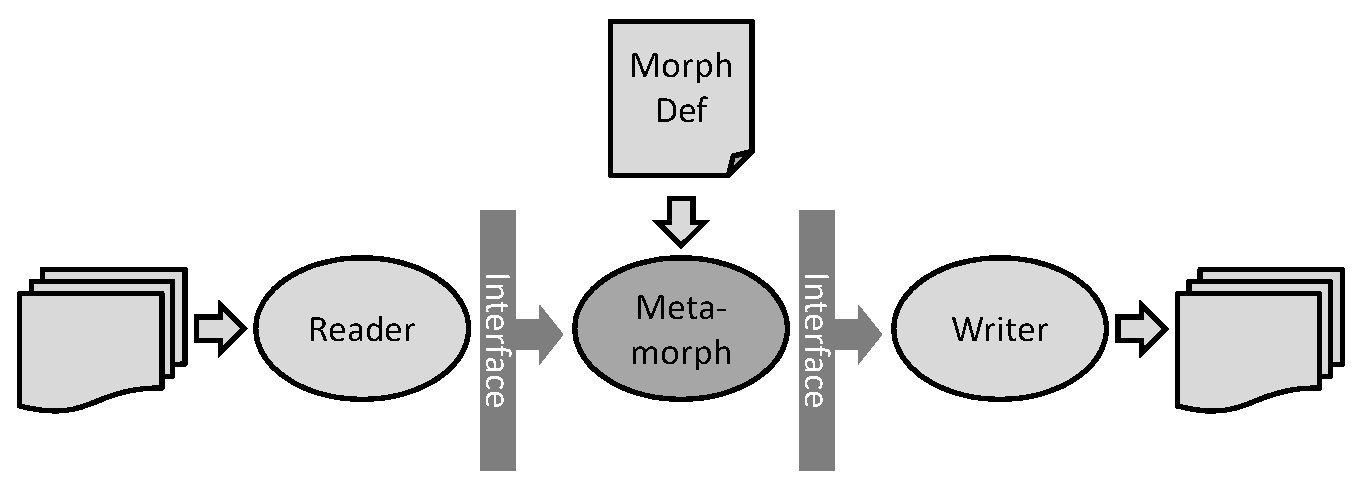
\includegraphics[width=.70\textwidth]{figures/readerwriter}
\caption{A typical processing pipeline including a Metamorph object for data transformation.}\label{fig:readerwriter}
\end{figure}


This section explains the how such a setup is implemented in practice. Subsection \ref{java} is dedicated to the Java code needed to wire the pipeline parts together, subsection \ref{def_lang} focuses on the Metamorph definition language. 


\subsection{The Java Side}\label{java}

The follwing subsection explain how to create a Metamorph object, how to build a processing pipeline and how to handle exceptions.

\subsubsection{Creation}

A new Metamorph is created by calling {\tt build()} on MetamorphBuilder. See listing \ref{creation}. Please note that the Metamorph object is not thread-safe. 

\begin{lstlisting}[float=htb, label=creation, caption=Creating a Metamorph object based on a Metamorph description., language=Java]
final Metamorph metamorph = MetamorphBuilder.build("definition.xml");
\end{lstlisting}

\subsubsection{Wiring}
The Metamorph object acts as a pipe element in the data stream. See also figure \ref{fig:readerwriter}. This means that we must wire it to a data source (or reader) and a data sink (or writer). Listing \ref{codepipeline1} shows how. First all elements of the processing chain are created.
The wiring is done by calling {\tt setReceiver()}. The call returns its argument, preserving the respective type. Thus the calls can be chained to build up a pipeline as shown in the listing. Finally the processing is stared by calling the respective method on the data source/reader. The method name depends on the reader. In the Metamorph project {\tt read()} is used by convention.

\begin{lstlisting}[float=htb, label=codepipeline1,caption= Putting together a processing pipeline according to the pattern in section \ref{pipeline}., language=Java]
// create neccessary objects
final PicaReader reader = new PicaReader();
final Metamorph metamorph = MetamorphBuilder.build("defnition.xml");
final ListMapWriter writer = new ListMapWriter();

//wire them
reader.setReceiver(metamorph).setReceiver(writer);

//start processing
reader.read(input);

\end{lstlisting}

Listing \ref{codepipeline2} shows a few more sophisticated wiring patterns, such as adding an additional element, junctions or splitters.

\begin{lstlisting}[float=htb, label=codepipeline2,caption= Advanced wiring., language=Java]
//add logging
reader.setReceiver(new LogPipe()).setReceiver(metamorph).setReceiver(writer);

//adding a tee junction
reader.setReceiver(new Tee()).setReceivers(writer1, writer2);

//splitting based on a metamorph description
final Splitter splitter = new Splitter("morph/typeSplitter.xml");
reader.setReceiver(splitter).setReceiver("Tn", writer1);
splitter.setReceiver("Tp", writer2);
\end{lstlisting}


\subsubsection{Error Handling}
If an exception occurs during the processing of a stream of records, it is back propagated to the first element in the chain. This normally means that processing is terminated which may not be the preferred action. Imagine processing a million records. One normally prefers to log any error but continue the processing.
For this reason an error handler may be registered with the Metamorph object. It catches all exceptions occurring in the Metamorph object and below. Listing \ref{errorhandling} shows the respective code snippet.  
\begin{lstlisting}[float=htb, label=errorhandling,caption= Registering an error handler., language=Java]
metamorph.setErrorHandler(new MetamorphErrorHandler() {
	@Override
	public void error(final Exception e) {
		// TODO fill in your error handling code
	}
});
\end{lstlisting}


\subsection{Metamorph Definition Language}\label{def_lang}
The transformation a specific Metamoph instance performs are defined in a Metamorph definition in XML. See also figure \ref{fig:readerwriter}. The structure of the XML is constrained by a schema ({\tt metamorph.xsd}). Listing \ref{morphdef} shows the high level organization of a Metamorph definition.

\begin{lstlisting}[float=htb, label=morphdef,caption=Structure of a Metamorph definition file.]
<?xml version="1.0" encoding="UTF-8"?>
<metamorph xmlns="http://www.culturegraph.org/metamorph"
	xmlns:xsi="http://www.w3.org/2001/XMLSchema-instance"
	xsi:schemaLocation="http://www.culturegraph.org/metamorph metamorph.xsd"
	entityMarker="." version="2">
   <meta><!-- Metadata --></meta>
   <functions><!-- Function definitions --></functions>
   <rules><!-- Transformation rules --></rules>
   <maps><!-- Data maps --></maps>
</metamorph>
\end{lstlisting}
The root element {\tt metamorph} has two attributes: One indicates the Metamorph version the document it intended to work with, the second indicates the character used to separate entity names (see also section \ref{dispatching}). Within the {\tt metamorph} tag there are four sections.
The first and optional one holds metadata for the definition file. The second section -- also optional -- holds definition of custom functions. See section \ref{customfunc}.
The {\tt rules} block defines the actual transformation rules. All of the following subsection refer to them.
Finally the optional {\tt maps} block allows to define maps/dictionaries for lookup functionality. See section \ref{lookup} for details.


\subsubsection{Receiving Pieces of Data}\label{data}

The {\tt data} tag is used to receive literals. Use the {\tt source} attribute to address the literal you want to catch. Listing \ref{lst:data} would receive the value of any literal with name {\it literalname}, enclosed in an entity named {\it entityname}.
The value is then sent to the downstream {\tt StreamReceiver} under the name {\it newName}. It is thus the most basic form of mapping data.
\begin{lstlisting}[float=htb, label=lst:data,caption=Receiving values from literals]
<data source="entityname.literalname" name="newName" />
\end{lstlisting}


\subsubsection{Processing Pieces of Data}\label{process}
After picking up a literal, its content can be processed sending it to the downstream {\tt StreamReceiver}.
Processing steps are added inside the {\tt data} tag. Listing \ref{lst:process} shows an example in which the date of death of an author in the PND is extracted from the Pica records and renamed to the corresponding RDF property (for the complete mapping description see the DNB linked data service documentation).
\begin{lstlisting}[float=htb, label=lst:process,caption=Processing data within the {\tt data} tag]
<data name="rdaGr2:dateOfDeath" source="032Aa.a">
  <replace pattern=" " with="" />
  <regexp match="-((\d*?))$" format="${1}" />
</data>
\end{lstlisting}

In the PND birth and death of an author are stored both in one subfield (literal in Metamorph speak) in the form 'birth - death' . So the need for processing arises.
First we eliminate all whitespaces by using a {\tt replace} operation. Next we apply regular expression matching {\tt regexp} and extract the firs match group ({\$\{1\}}) corresponding to the year of death.

Please note that functions may return zero to $n$ values. If no value is returned, the processing is stopped and nothing will be sent downstream. If for instance a {\tt regexp} does not match, processing stops and there will be no 'rdaGr2:dateOfDeath' in the output stream.

Builtin functions include:
{\tt compose}, {\tt constant}, {\tt count}, {\tt regexp}, {\tt replace}, {\tt substring}, {\tt lookup}, {\tt whitelist}, {\tt blacklist}, {\tt isbn}, {\tt equals}, {\tt htmlanchor}, {\tt trim}, {\tt split}, {\tt normalize-utf8} and {\tt occurence}. For the time being, see the test-cases and {\tt schema/metamorph.xsd} for arguments and usage examples.



\subsubsection{Looking up  Pieces of Data}\label{lookup}

A certain group of functions takes a map/dictionary as argument: {\tt lookup}, {\tt whitelist}, {\tt blacklist} etc.
In this section the usage of such maps will be explained. We start with a simple example of data lookup.

\paragraph{Local Lookup}

Take for instance an operation in which you want to replace values according to a lookup table: Value 'A' maps to 'print', 'B' maps to 'audiovisual' an so forth. This is accomplished by the {\tt lookup} function. The lookup table is defined inside the {\tt lookup} tag. Listing \ref{simplelookup} depicts this situation.

\begin{lstlisting}[float=htb, label=simplelookup,caption=Performing a simple lookup operation]
<data source="002@.0" name="dcterms:format">
  <substring start="0" end="1" />
  <lookup>
    <entry name="A" value="print" />
    <entry name="B" value="audiovisual" />
    <entry name="O" value="online" />
  </lookup>
</data>	
\end{lstlisting}

\paragraph{Maps}

The same lookup tables may used in different places in a Metamorph definition. To enable reuse, a map/dictionary can be defined separately from the respective lookup function. In the following listing the {\tt lookup} function refers to the table using the name {\it material}. Later in the code the actual map is defined using the {\tt map} tag. See listing \ref{maps}.

\begin{lstlisting}[float=htb, label=maps,caption={Defining a standalone map, which can be independently addressed by different lookup functions.}]
[...]
<lookup in="material">
[...]
<map name="material">
  <entry name="A" value="print" />
  <entry name="B" value="audiovisual" />
  <entry name="O" value="online" />
</map>
\end{lstlisting}

\paragraph{External Data Sources}

The situation might arise that the data used in lookup operations cannot be hardcoded in xml; or at least hard-coding it would be inconvenient. Imagine we want to resolve author ids to author names: Putting all the id-name mappings into the Metamorph definition file is certainly not desirable.
To address this issue, any data source implementing the {\tt Map} interface can be connected to the {\tt Metamorph} object as shown in listing \ref{regdata}. The data is referenced in the Metamorph definition file by '{\it name of map}'.

\begin{lstlisting}[float=htb, label=regdata,caption= Registering a map with the metamorph object., language=Java]
//create a Map. Any object implementing Map<String, String> will do
final Map<String, String> map = new HashMap<String, String>();
map.put("one key", "first String");
map.put("another key", "another String");

//tell metamorph to use it during lookup operations
metamorph.putMap("name of map", map);
\end{lstlisting}



\subsubsection{Integration of custom Java code}\label{customfunc}

If the predefined functions for data processing do not satisfy your needs, you may define new functions as shown in listing \ref{def}.
In the definition statement a Java class is bound to a name which is subsequently used to refer to it. There are a few important points to note:
The class must implement the {\tt Function} interface. For each attribute provided when referencing the function, a respective {\tt set} method is called right after instantiation. This mechanism correctly handles the types {\tt String}, {\tt boolean} and {\tt int}. A function is instantiated once per use in Metamorph definition and may thus maintain a state. See the JavaDoc for more details, examples and advanced issues such as dealing with state.

\begin{lstlisting}[float=htb, label=def,caption=User defined functions.]
<functions>
   <def name="my_super_function" class="org.myorg.myfunctions.MySuperFunction" />
</functions> 
\end{lstlisting}


\subsubsection{Recursion}\label{recursion}

Pieces of data processed with Metamorph are by default sent to the {\tt StreamReceiver} registered with Metamorph. There is however the posibillity to send a piece of data into a feedback loop. In this case the data reenters Metamorph just as it came from the upstream {\tt StreamSender}. This recursion is accomplished by prepending an '@' to the name of the data as shown in listing \ref{lst:rec}. 

\begin{lstlisting}[float=htb,label=lst:rec,caption=Prepending '@' to the literal name to enable recursive processing.]
<data source="002@.0" name="@format">
   <!--  processing -->
</data>

<!--  catch the data -->
<data source="@format" name="dcterms:format">
\end{lstlisting}

This pattern comes in handy when a piece of data is needed at several other places after preprocessing. It relieves you from copying and pasting the same preprocessing steps. It also improves efficiency as Metamorph will perform the preprocessing only one. Be careful though not to build infinite loops by forgetting to rename the data (removing the '@') in the final processing step.

\subsubsection{Collecting Pieces of Data}\label{collect}

In the case that an output depends on the values from more then one literal, we need to collect literals. Collectors are defined under the {\tt rules} tag, just as {\tt data} tags. Put {\tt data} tags inside the respective collectors to indicate which literals are to be collected. The following paragraphs briefly introduce the different collectors available. Note that all types of collectors except {\tt entity} can be nested, and that post-processing steps can be added by using the {\tt postprocess} tag. 


\paragraph{Combine}

is used to build one output literal from a combination of input literals. The  example in listing \ref{lst:combine} for instance collects the sur- and forename which are stored in separate literals to combine them according to the pattern 'surname, forename'.
There are several important points to note: By default {\tt combine} waits until all at least one value from each {\tt data} tag is received. If the collection is not complete on record end, no output is generated. After each output, the state of {\tt combine} is reset. If one {\tt data} tag receives literals repeatedly before the collection is complete only the last value will be retained.

\begin{lstlisting}[float=htb, label=lst:combine,caption=Combining data from two different data sources.]
<combine name="gnd:variantNameForThePerson" value="${surname}, ${forename}">
  <data source="028A.a" name="surname" />
  <data source="028A.d" name="forename"/>
</combine>
\end{lstlisting}

The standard behavior of {\tt combine} can be controlled with several arguments:
{\tt flushOn= "entityname"} generates output on the end of each entity with name {\it entityname}. Variables in the output pattern which are not yet bound to a value, are replaced with the empty string. Use {\tt flushOn="record"} to set the record end as output trigger.
{\tt reset="false"} disables the reset after output.
{\tt sameEntity="true"} will reset the {\tt combine} after each entity end and thus enforce combinations stemming from the same entities only. Note that the implementation only executes a reset if actually needed. Using {\tt sameEntity="true"} has thus no negative impact on performance.

\paragraph{Concatenate}
collects all received values and concatenates them on record end. {\tt flushOn= "entityname"} can be used to concatenate at the end of entity {\it entityname}.

\paragraph{Choose}
collects all received values and emits the most preferred one on record end. Preference is assigned according to the order the data sources appear within the {\tt choose} tag.  Eligible arguments are {\tt sameEntity} and {\tt flushOn}.

\paragraph{Group} is syntactic sugar. Use it to set name, value or both once for an entire group of {\tt data} or collect ({\tt combine}, {\tt choose}, etc. ) tags.

\paragraph{Entity} collects literals to rearrange them as an entity. Use the argument {\tt name} to assign a name to the entity. Further arguments are {\tt sameEntity}, {\tt flushOn} and {\tt reset}.

\paragraph{}For the time being, see the test-cases and {\tt schema/metamorph.xsd} for more information.

\subsubsection{Splitting Metamorph Definitions for Reuse}

In a complex project setting there may be several Metamorph definitions in use, and it is likely that they share common parts. Imagine for instance a transformations from Marc 21 record holding data on books to RDF, and Marc 21 records hodling data on authors to RDF. Both make use of a table assinging country names to ISO country codes. Such a table should only exist once. To accomodate for such reuse, Metamorph offes an include mechanism based on XInclude. Listing \ref{xinclude} shows an example in which a {\tt map} is included.

\begin{lstlisting}[float=htb, label=xinclude,caption=Including further XML files into a metamorph definition.]
<!-- main metamorph definition -->				
[...]
<maps>
   <include href="src/test/resources/mymap.xml" parse="xml"
	 xmlns="http://www.w3.org/2001/XInclude" />
</maps>
[...]

<!-- mymap.xml -->
<?xml version="1.1" encoding="UTF-8"?>
<map name="island_map" xmlns="http://www.culturegraph.org/metamorph">
	<entry name="Aloha" value="Hawaii" />
</map>
\end{lstlisting}
Use the {\tt include} tag from the {\tt http://www.w3.org/2001/XInclude} namespace to insert an external xml file into your definition. The included file must be valid xml itself, containig syntactically valid tags from the Metamorph namespace.

\subsection{Tools}

\subsubsection{Testing Framework for Metamorph Definitions}

Testing Metamorph definition files nearly always follows a simple pattern. Given the respective definition and an input, a specific output is expected. This can easily be expressed in XML as illustrated in listing \ref{test}.

\begin{lstlisting}[float=htb, label=test,caption=XML test definition]
<metamorph-test version="1.0"
	xmlns="http://www.culturegraph.org/metamorph-test" 
	xmlns:mm="http://www.culturegraph.org/metamorph"
	xmlns:cgxml="http://www.culturegraph.org/cgxml">
   <test-case name="My Testcase1">
      <input type="text/x-cg+xml">
	<!-- Your test input goes here -->           
      </input>
      <transformation type="text/x-metamorph+xml">
          <!-- the metamorph definition you want to test goes here  -->   
      </transformation>
      <result type="text/x-cg+xml">
          <!-- the expected result goes here  -->  
      </result>
   </test-case>
</metamorph-test>
\end{lstlisting}

How to integrate such a test definition written in XML into JUnit? JUnit feeds on Java classes. Thus we need to provide such a class as binding point. Listing  \ref{test_class} shows how.

\begin{lstlisting}[float=htb, label=test_class,caption= Binding XML test definitions to a test class., language=Java]
import org.culturegraph.metamorph.test.TestSuite;

@RunWith(TestSuite.class)
@TestDefinitions({"My Testcase1.xml", "My Testcase2.xml"})
public final class MyTest {/*bind to xml test*/}
\end{lstlisting}

The {\tt RunWith} annotation instructs JUnit to let {\tt org.culturegraph.metamorph.test.TestSuite} handle the testing.
Use the {\tt TestDefinitions} annotation to tell {\tt TestSuite} were to look for tests. If no such annotation is found {\tt TestSuite} looks for an XML files with the same name as the binding class. The XML files are expected to be located in the same folder as the binding class. The rationale is that both belong together and separating them would be confusing. Colocating the xml files with the class files is causing trouble with same build environments though. In the case of Maven there is an straight forward remedy: see listing \ref{maven_test}

\begin{lstlisting}[float=htb, label=maven_test,caption=Telling Maven not to ignore resources colocated with java files in the test source directory.]
<testResources>
   <testResource>
     <directory>src/test/java</directory>
        <excludes><exclude>**/*.java</exclude></excludes>	
   </testResource>
   <testResource>
      <directory>src/test/resources</directory>
   </testResource>
</testResources> 
\end{lstlisting}

An example test output in Eclipse is shown in figure \ref{fig:junit}. The root element is the binding class. Its children are the XML files, with the actual tests as leafs.

\begin{figure}[htp]
\centering
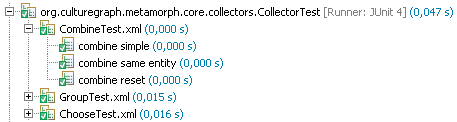
\includegraphics[width=.75\textwidth]{figures/junit}
\caption{Testcases shown in Eclipse}\label{fig:junit}
\end{figure}

\subsubsection{Visualizing Metamorph Definitions as Data Flow Diagramms}

The processing model behind Metamorph is that of a data flow. Hence it is straight forward to visualize Metamorph as a directed network representing this the resulting flow of data. Figure \ref{fig:match-title} shows such a visual representation. 

\begin{figure}[htp]
\centering
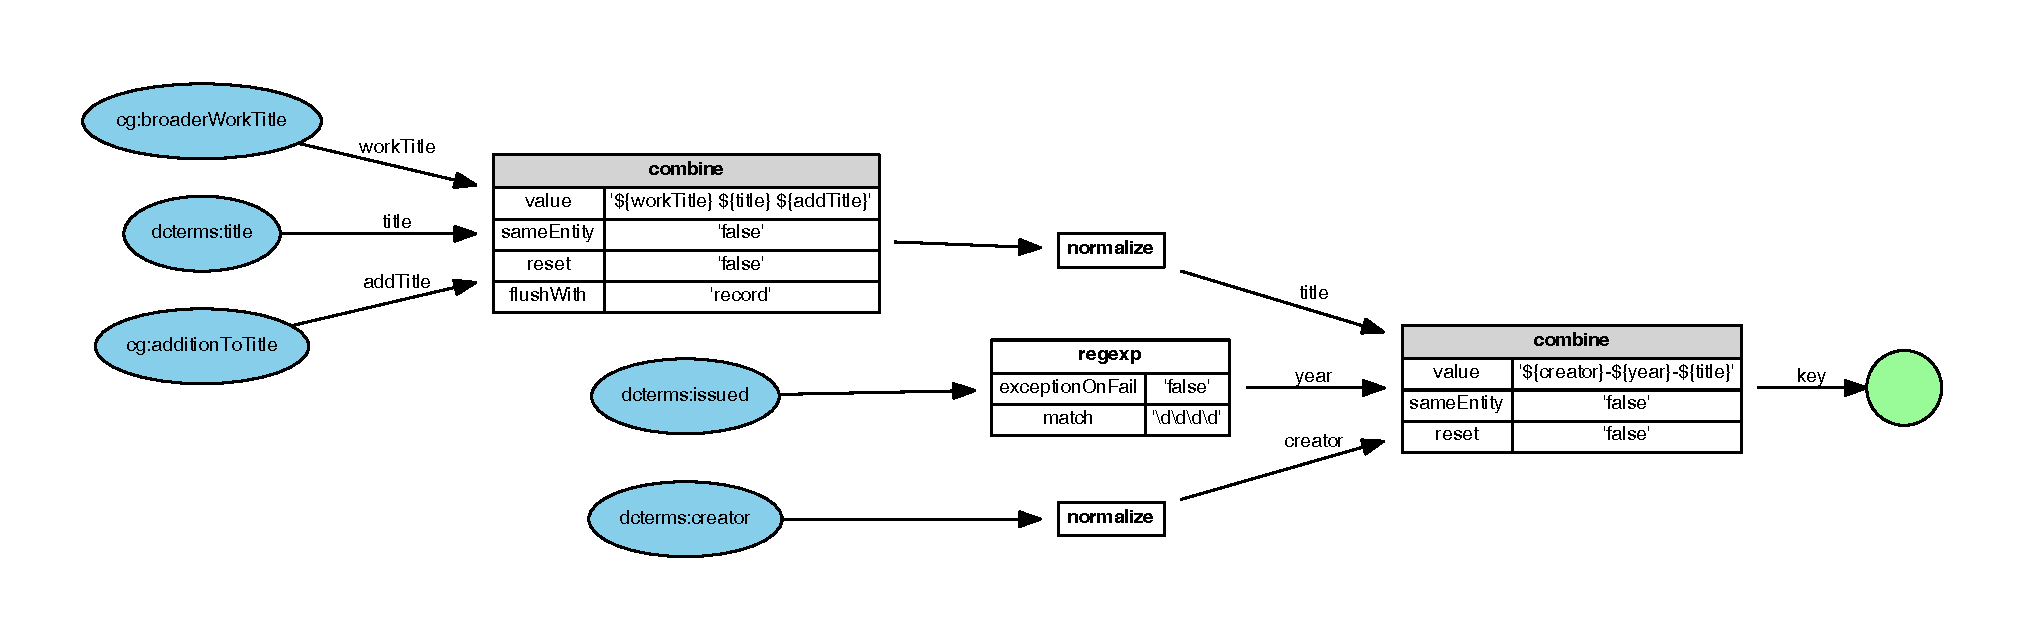
\includegraphics[width=1\textwidth]{figures/match-title}
\caption{Visualization of a Metamorph definition used in the Culturegraph project (see also section \ref{culturegraph})}\label{fig:match-title}
\end{figure}

Blue ellipses represent data sources while green circles represent data output. In our example we have a process with two combination stages and several functions applied to intermediate data. Stages in which data is collected are marked with a gray title bar showing the name of the operation. Functions are represented by white boxes. Both contain all parameters as name-value-lists. 
Two elements of Metamorph not shown in figure \ref{fig:match-title} are lookups and recursion. If lookup operations are included, the respective maps are depicted as gray tables. Finally, recursion (see section \ref{recursion}) is symbolized by yellow ellipses.

To visualize a Metamorph definition execute the class {\tt org.\-culturegraph.\-metamorph.\-Visualize}. The output is a graph description in the dot\footnote{See \url{http://www.graphviz.org/content/dot-language}} language. To generate a graphical representation any software compatible with the dot language can be used. The most obvious choice is Graphviz (\url{http://www.graphviz.org/}). 


\section{Application Examples}\label{apps}


\subsection{Culturegraph}\label{culturegraph}
Culturegraph is a Resolving- and Lookup-Service for bibliographic identifier. A Linked Open Data service that aims to establish shared identifiers for cultural works to ensure these resources can be reliably and persistently referenced.

From a technical view point, the following is happening: metadata from different sources is written to a database and matched to find correspondences. The matches and the original data are indexed and published on a web-portal. To accomplish this, metadata has to be transformed in various stages of the processing pipeline. Figure \ref{fig:flow} provides an overview.

\begin{figure}[htp]
\centering
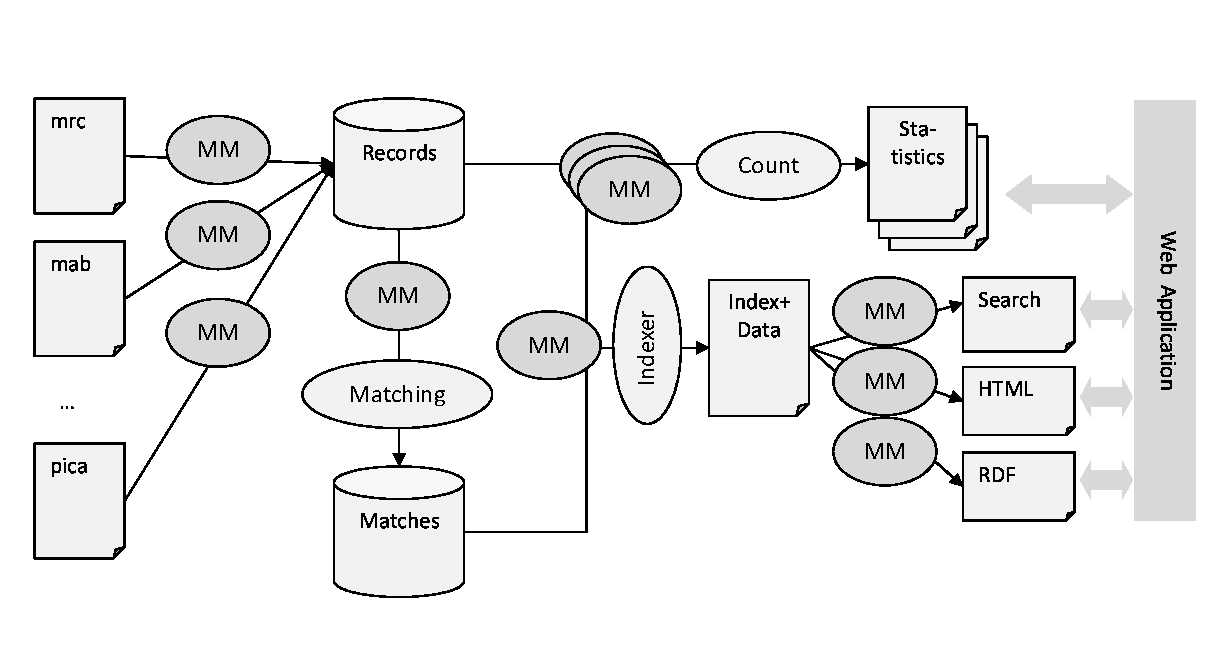
\includegraphics[width=.96\textwidth]{figures/flow}
\caption{Dataflows in Culturegraph. MM stands for a data transformation using Metamorph}\label{fig:flow}
\end{figure}


%\subsection{Linked Data Service DNB}


\section{Future Prospects}

\subsection{Open Issues and Limitations}

\subsection{Possible Extensions}
\subsubsection{Indexing Data}
\subsubsection{Writing RDF}

\end{document}

